\documentclass[main.tex]{subfiles}

\begin{document}
\chapter{Seasonal Trend Decomposition (STL)}
\label{chap:stl}
STL, as first described by Cleveland et al. \cite{stl}, is an
algorithm for decomposition of time series, which is a common task in
statistics and used by the BFAST algorithm to get the initial estimate of the
seasonal componenet $\hat{S_t}$.
STL decomposes a time series $Y_v$ into three components:
\[
Y_v = T_v + S_v + R_v \text{ for } v \in 1..N
\]
where:
\begin{itemize}
\item $T_v$ is the trend component, which captures the long-term progression of
  the time-series
\item $S_v$ is the seasonal component, which reflects the seasonal variation of
  the data
\item $R_v$ is the remainder(residual) component, which is the remaining variation of the time series
\end{itemize}
An example of such decomposition is illustrated on Figure \ref{fig_stl}.
STL alone, however, can not be used for break detection because it uses smoothing
that would temper with the breakpoint information.
\begin{figure}
  \centering
  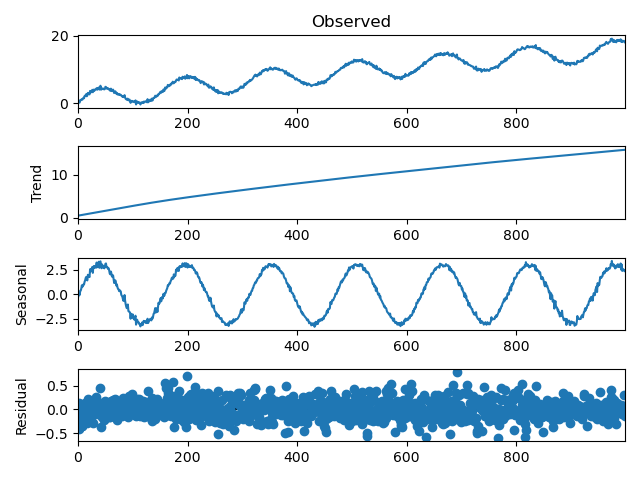
\includegraphics[width=0.7\textwidth]{imgs/stl1}
  \caption{STL applied to $f(x) = x^{0.75} + 2\sin(x)$ with added Gaussian noise
    $\sim \mathcal{N}(0, 0.25)$ and $n = 1000$. It can be seen that
    $T_v \approx v^{0.75}$, $S_v \approx 2\sin(v)$ and $R_v \sim \mathcal{N}(0, 0.25)$. }
  \label{fig_stl}
\end{figure}


\section{Locally Weighted Regression (LOESS)}
\label{sec:locally_weighted_running_line_smoother}
The key component of the STL method is the Locally Weighted Regression (LOESS),
that is described in \cite{loess} and \cite{stl}. LOESS is a robust smoothing method that is
commonly used in statistics and operates as follows:
\begin{itemize}
\item We have a set of $(x_i, y_i)$ for $1 \leq i \leq n$.
\item We wish for all $x$ fit a curve $\hat{g}(x)$ by giving the other points $x_i$ a
  weight $v_i$.
\item We select a value of $q \in \mathbb{Z}^+$
\item Let $\lambda_q(x)$ be the distance from $x$ to q'th farthest $x_i$.
  This definition would not, however, work when $q > n$. In that case, we must
  apply scaling by setting:
  \[
  \lambda_q(x) = \frac{q \cdot \lambda_n(x)}{n}
  \]
\item We calculate the weights using the tricube weight function:
  \[
  v_i = \left( 1 - \left( \frac{| x_i - x |}{\lambda_q(x)}  \right)^3\right)^3
  \]
  we also add a low shelf, for $| x_i - x | \geq \lambda_q(x)$, we set $v_i = 0$
\item We then use locally-linear or locally quadratic fitting with weights
  $\rho_i v_i$, where $\rho_i$ are the robustness weights, used by the STL.
  Addition of $\rho_v$ is crucial, since it allows us to ignore the outliers
  in the dataset and in this way introduce robustness into STL.
  The value of locally-fitted polynomial at $x$ is $\hat{g}(x)$, and $d$ is
  the degree of the fitted polynomial.
\end{itemize}
In this algorithm, $q$ is the smoothing factor. The higher the value of $q$ is, the more
the curve resembles a fitted polynomial of degree $d$ for all $x$. Another
important parameter is the value of $d$. Cleveland et al.
\cite{stl} suggest using $d \in \{1,2\}$ for STL. Value of $2$ is used when the
function of interest has a more pronounced curvature. An example of the usage of
LOESS smoothing can be seen on Figure \ref{fig_loess}.

\begin{figure}
  \centering
  \begin{subfigure}[b]{0.49\textwidth}
    \centering
    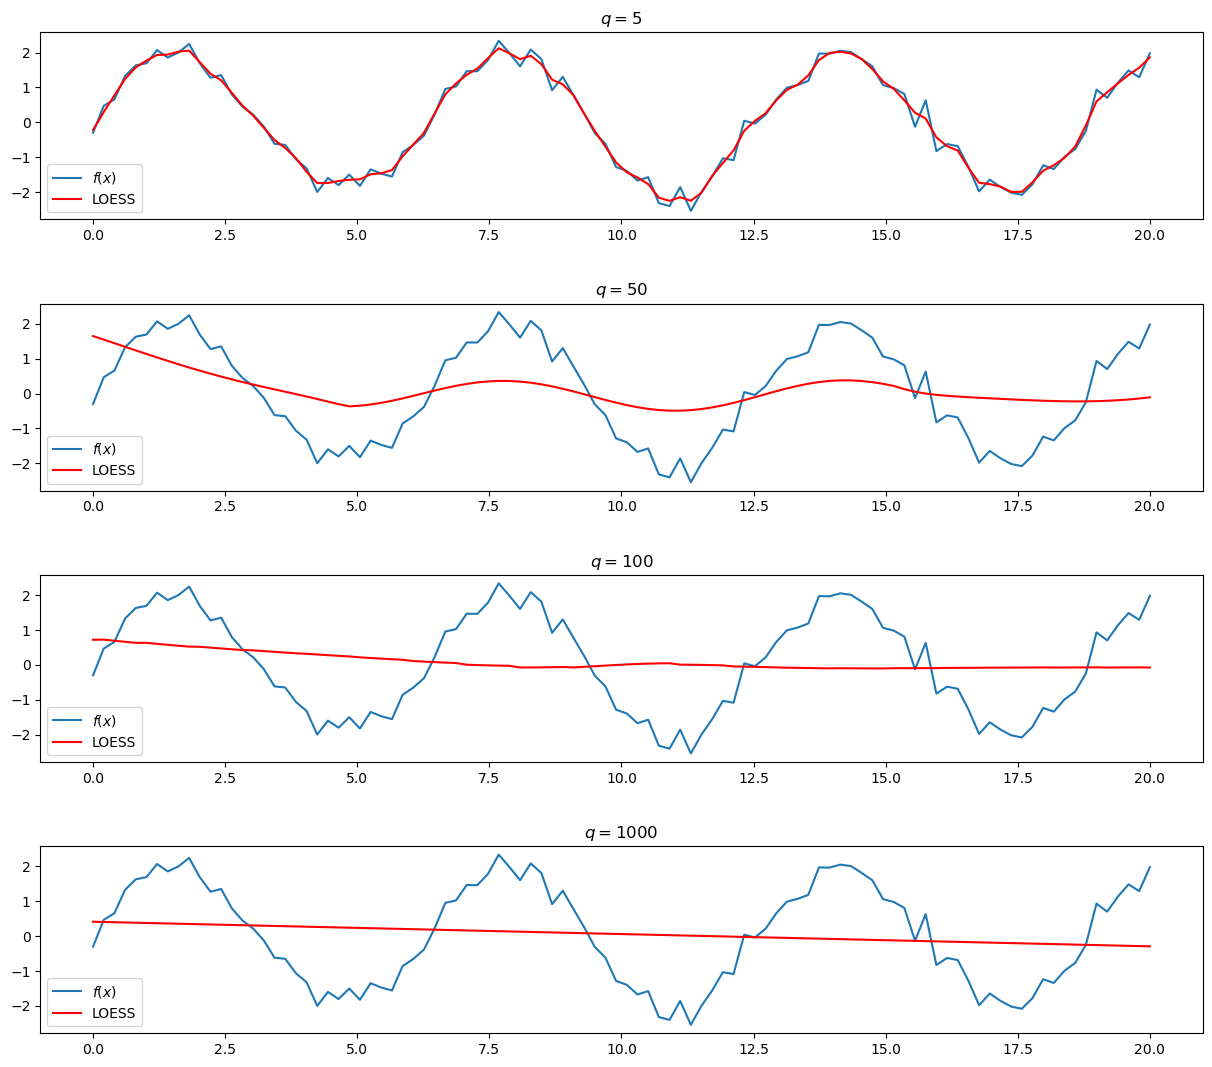
\includegraphics[width=\textwidth]{imgs/loess1}
    \caption{$d=1$}
  \end{subfigure}
  \begin{subfigure}[b]{0.49\textwidth}
    \centering
    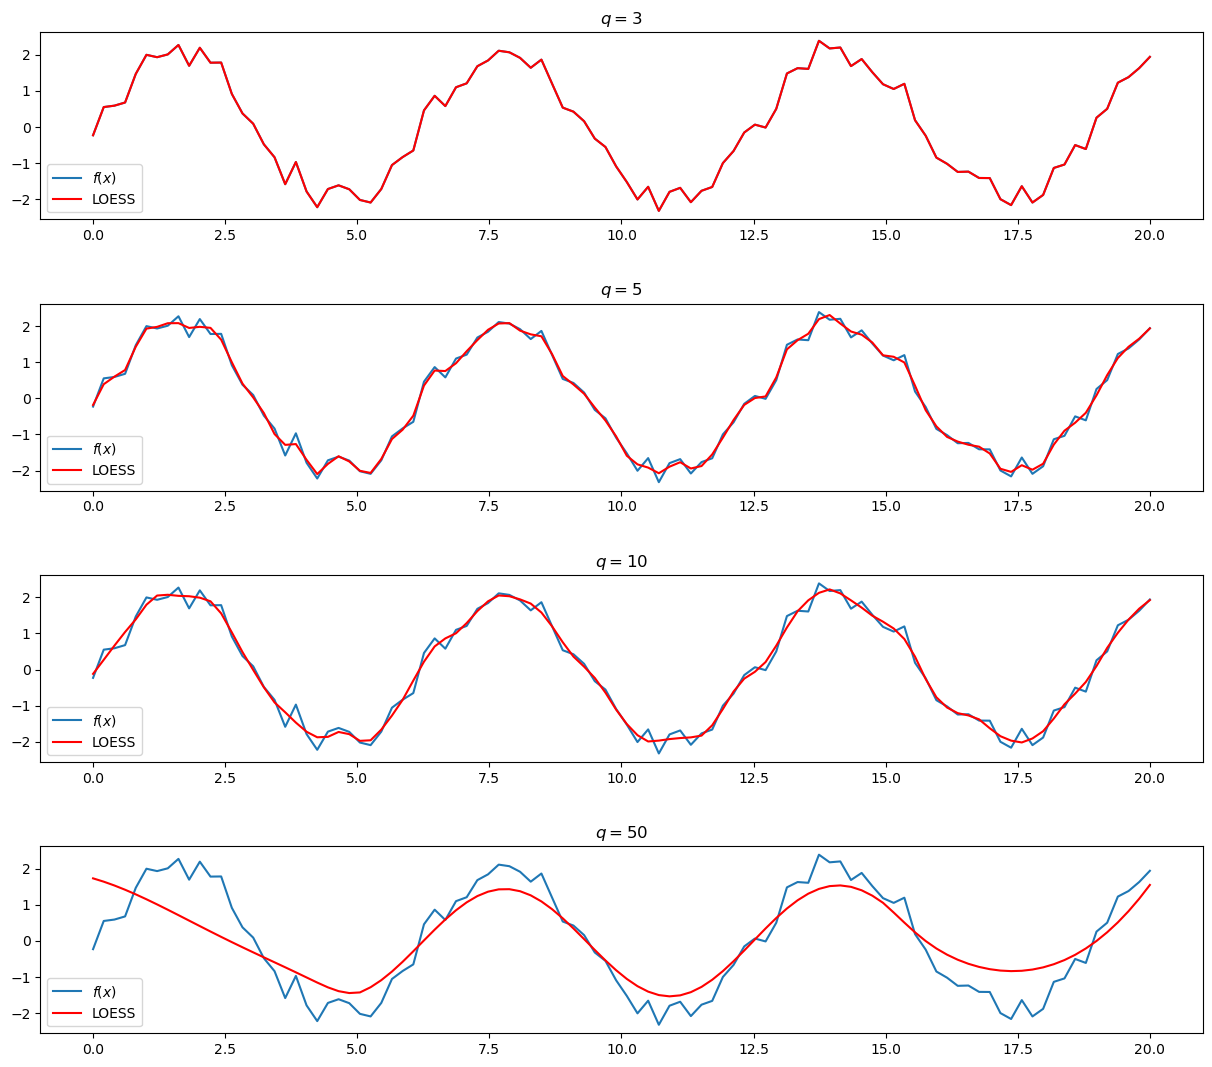
\includegraphics[width=\textwidth]{imgs/loess2}
    \caption{$d=2$}
  \end{subfigure}
  \caption{LOESS applied to $f(x) = 2\sin(x)$ with added Gaussian noise and $n = 100$}
  \label{fig_loess}
\end{figure}

\section{The Incremental Algorithm}
\label{sec:the_incremental_algorithm}
STL is performed through two nested loops and we begin by setting:
\begin{align*}
  T_v^{0} &= 0\\
  R_v^{0} &= 0\\
  \rho_v &= 1
\end{align*}
\subsection{Inner loop}
\label{subsec:inner_loop}
The inner loop consists of following steps:
\begin{enumerate}
\item \textbf{Detrending}:
  $Y_v - T_v^k$, where $k$ is the iteration number. Note however,
  that if a value of $Y_v$ is missing, the detrending value must also be missing.
\item \textbf{Cycle-Subseries Smoothing}:
  $Y_v - T_v^k$ is split into cycle-subseries. LOESS with $q=n_s$ and $d=1$ is
  applied to each cycle-subseries, resulting in $C^{k+1}$.
\item \textbf{Low-pass Filter of Smoothed Cycle-Subseries}:
  Apply the low-pass filter to $C_{k+1}$. This is accomplished by application of two
  moving averages of lag equal to 3 followed by LOESS smoothing with $q=n_l$
  and $d=1$.
  The result is saved as $L^{k+1}$
\item \textbf{Detrending of the Smoothed Cycle-Subseries}:
  $S^{k+1} = C^{k+1} - L^{k+1}$
\item \textbf{Deseasoning}:
  $Y_v - S_v^k$. If a value of $Y_v$ is missing, the detrending value must also be missing.
\item \textbf{Trend Smoothing}:
  Apply LOESS to $Y_v - S_v^k$ with $q = n_t$, resulting in $T^{k+1}$
\end{enumerate}

\subsection{Outer loop}
\label{subsec:outer_loop}
The outer loop consists of following steps:
\begin{enumerate}
\item Run the inner loop
\item Find the remainder:
  $R_v = Y_v - T_v - S_v$
\item Calculate the robustness weights from the remainder component:
  \[
  \rho_{v}= B\left( \frac{|R_v|}{6\cdot\text{median}(|R_v|)} \right)
  \]
  where $B$ is the bisquare weight function:
  \[
  B(x) =
  \begin{cases}
    \left(1-x^{2}\right)^{2} & \text{ for } 0 \leqslant x<1 \\
     0                     & \text{ for } x>1
  \end{cases}
\]
\end{enumerate}

\section{Parameters and Their Values}
\label{sec:parameter_values}
STL has following parameters \cite{stl}:
\begin{enumerate}
\item $n_p$ : period of the seasonal component in number of observations.
  Specific for each data set.
\item $n_i$ : number of inner loop iterations. \texttt{stlplus}, which is
  popular STL library that is used in the BFAST R implementation \cite{bfast-github}, uses a
  value of $n_i = 2$ \cite{stlplus}.
\item $d$: degree for the polynomials that is being fitted.
  \texttt{stlplus} uses a value of $d=1$ for all smoothing.
\item $n_o$ : number of the outer loop iterations. The default value in
  \texttt{stlplus} is 0. This can be adjusted if outliers are present in the dataset.
\item $n_l$ : value of the smoothing parameter ($q$) for the LOESS procedure in the
  \textbf{Low-pass filter} stage of the inner loop. Typically (which includes
  \texttt{stlplus}), $n_l$ is the smallest odd integer greater than the period.
\item $n_t$ : value of $q$ for the trend component, which should be odd.
  \texttt{stlplus} uses following:
  \[
  n_t =\text{nextodd}\left(
  \ceil[\bigg]{
    \frac{1.5 \cdot n_p}
         {1-1.5/n_s}
  }
  \right)
  \]
\item $n_s$ : value of $q$ for the seasonal component. According to Cleveland
  et al. \cite{stl}, it must be specifically and
  carefully chosen for each application. \texttt{stlplus} allows
  the user to select $n_s = \text{``\emph{periodic}''}$, which is, according to
  the package documentation \cite{stlplus}, equivalent to replacing
  the smoothing in the seasonal component with taking the mean. It is the value,
  used by the BFAST R-implementation.
\end{enumerate}
\biblio
\end{document}
